 \title{Lab 3: Humidity, Pressure, Acceleration Sensing}
\author{Engineering 100-950}
\date{Winter 2020}
\documentclass[12pt]{article}
\usepackage[margin=1in]{geometry}
\usepackage{fancyhdr}
\chead{Written and Edited by Arun Nagpal, Aaron Ridley, Scott Smith, Lyndon Shi, and Kitty Ascrizzi}
\usepackage{graphicx}
\usepackage{hyperref}

\begin{document}
	\maketitle
	\thispagestyle{fancy}
	\section*{Materials}
	\begin{itemize}
	    \item 1 \quad TMP36 Temperature Sensor
	    \item 1 \quad B57164K Amtherm Thermistor
		\item 1 \quad HIH-4030 Humidity Sensor
		\item 1 \quad MPX4115A Pressure Sensor
		\item 1 \quad ADXL335 3-Axis Accelerometer
        \item 2 \quad Arduino Nanos
        \item 1 \quad OpenLog
        \item 1 \quad Level-Shifter
        \item 1 \quad 1 k$\Omega$ Resistor
	\end{itemize}
	
	\section*{YouTube Video}
	\href{https://www.youtube.com/watch?v=uCouP3qL1oc}{Feel free to watch the YouTube video at this link (click here). It will help you understand how to calibrate the sensors used in this lab. The video uses the convenient analogRead() to voltage conversion, which is not what we want. We will want to use the technically accurate method in this lab: analogRead() * 5/1024.}

	\section*{Introduction}
	Recall the calibration of the TMP36 temperature sensor in last week's lab. You performed a \textbf{two-point calibration} where you assumed the calibration curve of the sensor was linear. Many sensors, like the ones you are using in this course, are actually \textbf{integrated circuits} (ICs). They process the raw measurement internally before it is outputted using a network of \textbf{transistors}, or electrical switches. This results in a linear or near-linear calibration curve that only needs to be adjusted parametrically.\\
	
	In this lab, you will lay out the rest of the sensors on the balloon payload system, and run some basic MATLAB processing scripts on your as of yet un-calibrated data. By the end of the lab, you will have built the majority of the sensing architecture of your payload.
	
	\section{Humidity, Pressure, and Temperature Sensors}
	We recommend you split your team in half and do parts 1 and 2 simultaneously, using two breadboards and two Arduinos. However, we recommend that you ensure the entire team knows how the system works as a whole at the end of the lab. Briefly discuss your sensors and how they work with your teammates at some point.
	
	\subsection*{Humidity Sensor}
	\begin{enumerate}		
		\item Identify the different pins on the humidity sensor from the spec.
		
		\item Connect your TMP36 temperature sensor like you have in previous labs and verify that you can record output. We will be printing to the Serial monitor (i.e. Serial.print) in this lab.
		
		\item Keep your temperature sensor circuit assembled and now also connect the humidity sensor to your Arduino. 
		
		\item Verify that you can record output from both sensors as well as time. Organize your output using comma-separated voltage values, and label each value by writing a line such as  ``Time, Temperature, Humidity" at the top of your output so you can identify which variable is which. 
		
		\item Take measurement data indoors and another measurement outside. Create calibration curve equations for both the temperature sensor and the humidity sensor. Write an Arduino program to test and make sure it works. The program should read the sensor's value once per second and output the values to the Serial monitor. Save this program, as you'll turn it in.
		
		\item Plot these curves in MATLAB with the x-axis in volts, and the y-axis in Celsius and \%RH for the temperature sensor and humidity sensor respectively. Plot these curves on separate figures. Include axis labels and a title.
	
	\end{enumerate}

		\begin{figure}[h]
			\begin{center}
				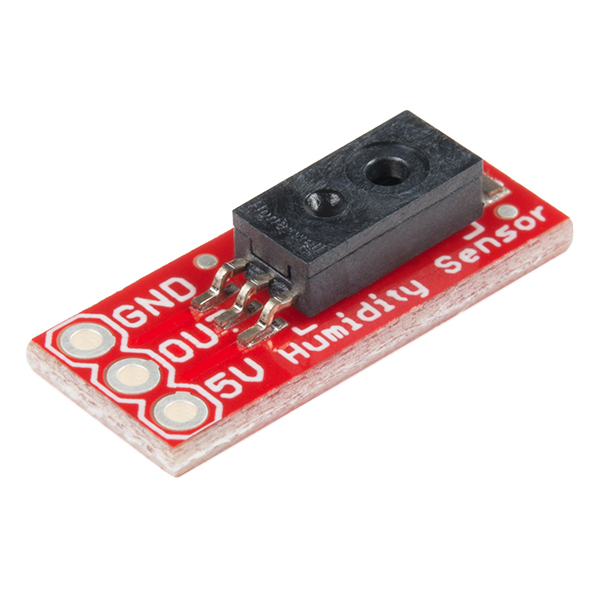
\includegraphics[scale=0.75]{Figures/HIH4030.jpg}
				\caption{The HIH-4030 Humidity Sensor}
			\end{center}
		\end{figure}
	
	\newpage
	\subsection*{Pressure Sensor}
	\begin{enumerate}
		\item Identify the different pins on the pressure sensor.
		
		\item  Connect the sensor to the Arduino, based on the pin-out on the spec and verify that you can record all output from all the sensors at the same time.
		
		\item Take a measurement and create a calibration curve equation for this sensor. Assume that a measurement of 0V maps to 0 pressure for the other measurement. Write an Arduino program to test it and make sure it works. The program should read the sensor's value once per second and output the pressure to the Serial monitor. Save this program, as you'll turn it in.
		
		\item Plot this curve, with the x-axis as volts, and the y-axis as pressure. Include a title and axis labels.
		
	\end{enumerate}

	\begin{figure}[h]
		\begin{center}
			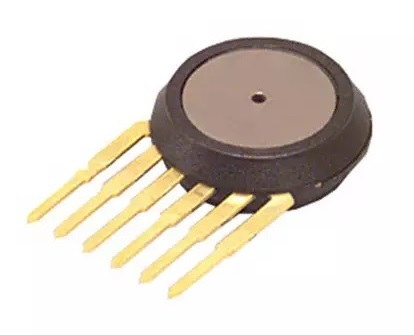
\includegraphics[scale=0.9]{Figures/MPX4115a.jpg}
			\caption{The MPX4115a Pressure Sensor}
		\end{center}
	\end{figure}
\subsection*{TMP36 and Thermistor}
On your board, integrate the TMP36 and Thermistor as per Lab 2. We will not calibrate these this week, since you learned how to do this last week. We will do final temperature calibrations later this semester in the cold chamber of the FXB. (See Lab 7 if you are curious!)

%------------------------------------------------
	\section{Accelerometer}
    
    Turning to the 3-axis accelerometer, you are going to try to calibrate the instrument using a fixed acceleration that you feel all of the time.
    
	\begin{enumerate}
		\item Identify the different pins on the accelerometer. Note that there are 3 output pins. \textbf{The accelerometer takes an input voltage of 3.3V.}
	
		\item Connect the sensor to the Arduino, based on the pin-out on the spec.
	
		\item Perform a two-point calibration for each of the three axes, and plot the calibration functions for all channels (axes) of the accelerometer in units of `g' on one plot. Make sure to label all axes, curves, and include a title in your graph. Write a program that reads the acceleration on every axis once every 10 ms, and outputs that data to the Serial monitor. Save this program, as you'll turn it in.
		
		\item Attach your OpenLog and Level-Shifter to your breadboard, and write a program to record acceleration data in 'g's for all axes, as well as time data, onto the SD card. Take measurements every 20 milliseconds. Test to make sure your program works, and delete all other files off of the SD card. Save this program, as you'll turn it in.
		
		\item Run your program and rotate your accelerometer such that every axis experiences the full acceleration of gravity, at both its positive and negative extremes. Try and get it so a few acceleration data points at each axis-extreme are due entirely to gravity (hold the accelerometer very still). Make sure the data is recorded correctly onto the SD card. If so, take this data and save it on your computer. Then, wipe the SD card.
		
		\item Now, shake your breadboard with the accelerometer rapidly for at least 10 seconds. Try safely exerting significant forces on all axes of the accelerometer, but don't dislodge pieces (like wires). Make sure this data is recorded onto the SD card. Take this data and save it onto your computer. Then, wipe the SD card.
		
	    \item Create two MATLAB graphs for the slowly turned accelerometer of step 5. In the first graph, plot x-acceleration vs z-acceleration on the x and y axes respectively. In the next graph, plot y-acceleration vs z-acceleration on the x and y axes respectively. 
	    
	    \item Repeat step 7, but now use the rapidly shaken data from step 6.  
		
	\end{enumerate}

	\begin{figure}[h!]
		\begin{center}
			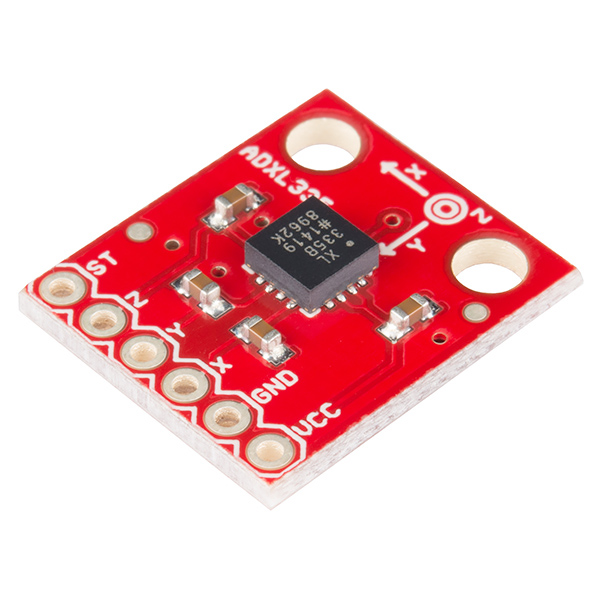
\includegraphics[scale=0.75]{Figures/ADXL335.jpg}
			\caption{The ADXL335 3-Axis Accelerometer}
		\end{center}
	\end{figure}

	\section*{Post Lab Questions}
	From now on, your entire group will submit one post lab assignment. Therefore, you should all collaborate on the post lab questions.
	
	\begin{enumerate}
		\item Draw a schematic that shows all of the components (TMP36 temperature sensor, pressure sensor, humidity sensor, Level-Shifter, OpenLog, and accelerometer) used today connected to a single Arduino. Make sure to include all of the relevant pins. This diagram should include all necessary connections like voltage inputs and ground lines as well as how information is transmitted. Clearly label the connections. This can be done by hand or in a computer tool, but it need to be very clear and easy to understand.
		
		\item Which of these three sensors (humidity, pressure, acceleration) do you think experiences the most variance as a function of temperature? Why?
		
		\item What do the different pins on the humidity sensor do? Explain Figures 3 and 4 on the spec, and how they relate to the calibration curve of the sensor. What is the sensor's nominal supply voltage?
		
		\item Your humidity sensor records values that generate a linear relationship of voltage to relative humidity within a particular temperature. As the temperature changes, the slope of your line can unfortunately change as well. It is possible to correct for this error by using an additional equation. You can find this equation in the spec sheet for the component. This corrected output is known as true relative humidity. State the equation and explain what each of the variables are.
		
		\item In an ideal situation, what should we hold constant while calibrating the humidity sensor?
		
		\item Calculate the absolute humidity by using the formula described at \href{https://carnotcycle.wordpress.com/2012/08/04/how-to-convert-relative-humidity-to-absolute-humidity/}{this link (click here).} Do this for the data measurement you took outside with the humidity sensor. Show your work.
		
		\item What is the maximum power that can be provided to the humidity sensor?
		
		(Hint: Power = Current * Voltage)
		
		\item What are the 3 unused pins on the pressure sensor for? Based on the nominal operating characteristics of the device, what is the maximum power that can be provided to the device?
		
		\item Explain concisely what the "sealed vacuum reference" mentioned in the pressure sensor spec is for. Does the sensor make an absolute or relative pressure measurement? What's the difference between the two?
		
		\item Brainstorm and come up with two processes related to the atmosphere or with balloons that an accelerometer can be used to measure. Justify your answers.
		
		\item What are your calibration points for your accelerometer, in units of ``g"s? How many total calibration point measurements do you need to perform for this sensor?
        
        \item What do you expect the maximum acceleration reading to be on the Arduino given the maximum allowed acceleration for the ADXL335 (see the spec sheet)? How does this compare with what you saw in your MATLAB plot for the rapidly shaken accelerometer?
        
        \item Analyze the MATLAB plot you made for the slowly turned accelerometer. What do you see? Did you manage to get to 1g on every axis? If not, how far off were you? What could have caused this discrepancy? 
        
        \item Describe the difference between an accelerometer and a gyroscope (you can find information online). Give two examples related to space technology for why you would want to use a gyroscope.
        
        \item Which of the sensors that we used today should be read the most frequently? Justify your answer, and consider the final project of the course in your response.
        
	\end{enumerate}
    
    
   \section*{Documentation for Postlab}
    From now on, one team member should submit documentation to represent the entire team. On Canvas, turn in the following files.
    \begin{enumerate}
        \item A PDF containing answers to the post lab questions and all graphs created in the lab (temperature calibration, humidity calibration, pressure calibration, accelerometer axes calibration, x vs. z and y vs. z for the slowly turned accelerometer, and x vs. z and y vs. z for the rapidly shaken accelerometer).
        \item All of the Arduino code (.ino) that was created for this lab (humidity sensor calibration, pressure sensor calibration, accelerometer calibration, and accelerometer to SD card).
        \item The MATLAB code (.mat) used to generate graphs in the lab.
    \end{enumerate}
\end{document}
